

\documentclass[tc_tp3_anexo_main.tex]{subfiles}

\begin{document}


\chapter{Filtro con GIC: respuesta al escal\'on}

Se realiz\'o una nueva medici\'on de respuesta al escal\'on, con el fin de observar el transitorio con m\'as detalle y contrastar los par\'ametros $\omega_d$ y $\alpha$ emp\'iricos con los te\'oricos.\par

La medici\'on efectuada fue sobre la salida correspondiente a una entrada cuadrada de $100Hz$ y $9.91V_{pp}$, y se puede observar a continuaci\'on:

\begin{figure}[H]
	\centering
	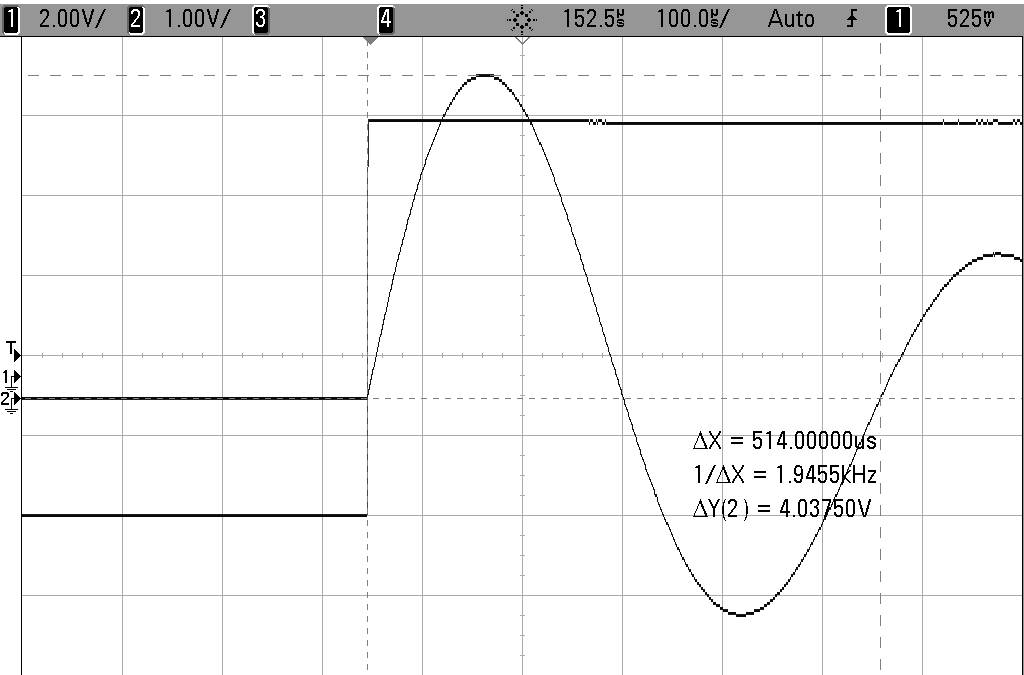
\includegraphics[scale=0.33]{fotosgic/gic_rtaesc.png}
	\caption{Respuesta al escal\'on medida}
\end{figure}

Como se puede observar, el pseudoper\'iodo medido es de $514\mu s$. Anal\'iticamente se hab\'ia determinado que el mismo deber\'ia ser de $486\mu s$, con lo cual el error del c\'alculo es de un $5.45\%$.\par 

Para obtener el factor de amortiguamiento se midi\'o tambi\'en la amplitud del segundo pico ($A_2$), de forma tal de poder determinar $\alpha$ a partir de su relaci\'on con $A_1$. Partimos de la expresi\'on anal\'itica de la respuesta en frecuencia:\par

\begin{equation}
	y(t) = u(t) \cdot \left(1+\frac{R_4}{R_8} \right) \cdot \frac{2\alpha}{\omega_d} \cdot e^{-\alpha t}\cdot \sin{\omega_d t} 
\end{equation}

Sabiendo que el primer m\'aximo corresponde a $t_1 = \nicefrac{T'}{4}$ y el segundo en $t_2 =5\cdot \nicefrac{T'}{4}$ (donde $T' = \nicefrac{2\pi}{\omega_d}$ es el pseudoper\'iodo), evaluando en estos tiempos se obtienen las amplitudes:\par 

\begin{equation}
	\begin{aligned}
		A_1 &=  \left(1+\frac{R_4}{R_8} \right) \cdot \frac{2\alpha}{\omega_d} \cdot e^{-\alpha \cdot \nicefrac{T'}{4}} \\
		A_2 &=  \left(1+\frac{R_4}{R_8} \right) \cdot \frac{2\alpha}{\omega_d} \cdot e^{-\alpha\cdot 5\cdot \nicefrac{T'}{4}} 
	\end{aligned}
\end{equation}

Por lo tanto, realizando el cociente entre ambas expresiones obtenemos que:

\[ \frac{A_1}{A_2}  = e^{-\alpha \cdot \nicefrac{T'}{4} + \alpha\cdot 5\cdot \nicefrac{T'}{4}}  = e^{\alpha \cdot T'} \]

Finalmente, el valor de $\alpha$ puede obtenerse a partir de las mediciones realizadas como:

\begin{equation}
	\alpha = \frac{1}{T'} \cdot \ln{\left(\frac{A_1}{A_2}\right)}
\end{equation}

Dado que los valores medidos fueron $A_1 = 4.0375V$ y $A_2 = 1.8125V$ y utilizando el $T'$ medido, se obtiene \textbf{$\alpha = 1558\nicefrac{rad}{s}$}. Por lo tanto, el error del valor calculado ($1629\nicefrac{rad}{s}$) es del $4.55\%$.\par

Estos valores de error son consistentes con el $6\%$ de error entre la frecuencia de resonancia medida y la calculada.

\end{document}
